Mehr zu MVP (Model-View-Presenter) kann man \textit{\textbf{in folgende Quelle}} lesen.

Model-View-Presenter Architektur wird in den Anwendungen benutzt, die eine Oberfläche besitzen.
Die Architektur teilt die Anwendung in 3 Teile:
\begin{itemize}
    \item \textbf{Model} - enthält die komplete Logik des Programms.
    \item \textbf{View} - empfängt alle Ereignisse von der Oberfläche und enthält die Daten, die angezeigt werden sollen.
    \item \textbf{Presenter} - transformiert die Daten in beide Richtungen vom Model zu View 
    und vom View zu Model
\end{itemize}


Eigenschaften der MVP Architektur:
\begin{itemize}
    \item \textbf{Presenter} und \textbf{Model} lassen sich mit Unittests abdecken.
    \item Jedes neues \textbf{View} braucht ein eigenes \textbf{Presenter}.
\end{itemize}


\begin{figure}[H]
    \centering
    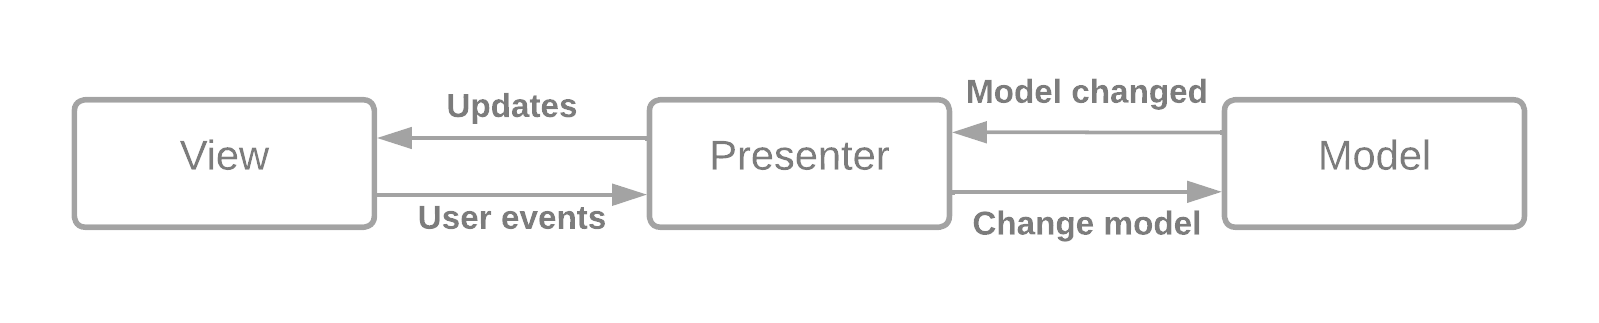
\includegraphics[width=1\textwidth]{./images/MVP.png}
    \caption[Datenfluss in MVP Architektur]{Datenfluss in MVP Architektur \footnotemark}
    \label{fig:MVP}
\end{figure}
\footnotetext{Eigene Quelle}